%% LyX 2.0.2 created this file.  For more info, see http://www.lyx.org/.
%% Do not edit unless you really know what you are doing.
\documentclass[oneside]{book}
\usepackage{prettyref}
\usepackage[utf8]{inputenc}
\usepackage{geometry}
\usepackage{pdfpages}
\usepackage{mdwlist}
\pagestyle{plain}

% \usepackage{lastpage} % for the number of the last page in the document
% \usepackage{fancyhdr}
% \pagestyle{fancy}
% \fancyhf{}
% \lhead{--- DRAFT ---}
% \rhead{Section \thesection}

\geometry{verbose,tmargin=2cm,bmargin=2cm,lmargin=2cm,rmargin=2cm}
\setcounter{secnumdepth}{3}
\setcounter{tocdepth}{3}
\usepackage[unicode=true,pdfusetitle,
 bookmarks=true,bookmarksnumbered=true,bookmarksopen=false,
 breaklinks=false,pdfborder={0 0 1},backref=section,colorlinks=true]
 {hyperref}

\setlength{\parskip}{\smallskipamount}
\setlength{\parindent}{0pt}

\makeatletter
%%%%%%%%%%%%%%%%%%%%%%%%%%%%%% User specified LaTeX commands.

\usepackage{sr}


\makeatother

\begin{document}

\tableofcontents{}

\pagebreak{}
\setcounter{secnumdepth}{-2}
\part{\label{DEFINITIONS}INITIAL PROVISIONS - DEFINITIONS}
\begin{enumerate}
\item ``Agenda'' means the order of business of a regular
or special meeting, as defined in the latest edition of Robert's Rules
of Order; \\
 ``By-Laws'' means the By-Laws of the Concordia
Student Union; \\
``campaign materials'' means any printed
matter, paid advertisement in any media, or any other object used
to promote or oppose, directly or indirectly, the election of a candidate,
or a particular option in a referendum, as the case may be; \\
``Chairperson'' means the Chairperson of
Council; \\
``Code'' means the Revised Code of CSU Standing
Regulations; \\
``Council'' means the Council of Representatives
of the Student Union; \\
``Council-Elect'' means the candidates elected
to Council in the Annual General Election who have not yet taken office;
\\
``day'' means a business day which excludes
Saturdays, Sundays, Good Friday, Easter Monday, third Monday of the
month of May, Quebec's National Holiday, Canada Day (or July 2nd if
July 1st falls on a Sunday), Labour day, Thanksgivings day, Concordia
University Holidays where the University is closed and any days starting
December 20th until January 5th inclusively. These days shall not
be calculated in calculating any delays under the By-Laws, regulations
or policies of the Student Union; \\
``Election'' refers to an electoral process
which begins with the announcement of the Poll by the Chief Electoral
Officer; \\
``Employee'' means a person employed by
the Student Union or its subsidiary, other than an Officer of the
Student Union or its subsidiary; \\
``Executives'' means a member of the Executive
of the Student Union;; \\
``Fee levy'' means any fee levied on members
and approved through referendum; \\
``general meeting'' means an annual, special,
or informational general meeting of the Student Union, as defined
in the By-Laws; \\
``general public notice'' means the placement
of posters in the following buildings: Administration/Central (AD/CC),
Hingston Hall (HA), Communication Studies \& Journalism Building (CJ),
Richard J. Renaud Science Complex (SP), Theatre and Dance Building
(TJ), Library Building (LB), Campus Centre (SC), Commerce and Administration
(GM), Hall (H), Engineering and Visual Arts (EV) and Visual Arts (VA)
buildings and an announcement on the CSU website; \\
``member'' means a person who fulfills the
conditions of membership under section 3.1 of the By-Laws; \\
``mutatis mutandis'' means ``with
the necessary changes''; \\
``office'' means the office of the President,
a Vice-President or the office of a Representatives for a particular
faculty, as the case may be, unless otherwise specified; ``ordinary
resolution or regulation''; regulation or resolution
requiring a majority vote at Council to be adopted; \\
``President'' means the President of the
Student Union; \\
``President-Elect'' means a candidate who
has been declared elected in the Annual General Election for the office
of the President, and who has not yet taken office; \\
``polling period'' means a period of 3 consecutive
school days during which the polls in an election or referendum open
at 10 a.m. and close at 8 p.m.; \\
``public notice'' means publication on the
Council electronic mailing list, the CSU website and placement of
posters on the Student Union bulletin board; \\
``referendum committee'' means a group recognised
as such by the Chief Electoral Officer for the purpose of promoting
a particular option in a referendum; \\
``regular meeting'' means a regular meeting
of Council as defined in the By-Laws; \\
``Representative'' means a duly elected
member of Council who has taken office; \\
``Secretary'' means the Secretary of Council;
\\
``special meeting'' means a special meeting
of Council, as defined in the By-Laws; \\
``student at large'' means a member who
is not a Representative, an Executive, the Chairperson or Council
Secretary, the Chief Electoral Officer or a member of the Judicial
Board; \\
``Student Union'' means the Concordia Student
Union; \\
``subsidiary'' means CUSACORP Management
Ltd. and its various operations; \\
``these regulations'' means the regulations
inside this Code \\
``in writing'' means either by a hard copy
or via electronic mail; \\
``University'' means Concordia University; 
\suspend{enumerate}
\setcounter{secnumdepth}{3}


\part{\label{COUNCIL_OF_REPRESENTATIVES}COUNCIL OF REPRESENTATIVES}


\chapter{\label{Council_Scope}Scope }

\resume{enumerate}

\item These regulations are adopted in accordance with section 6.3 of the
By-Laws. 
\item The regulations in this book apply to the Council of Representatives,
its committees and other subsidiary bodies, and the proceedings thereof. 

\suspend{enumerate}
\chapter{\label{Composition_of_Council}Composition of Council }
\resume{enumerate}
\item In accordance with the By-Laws, the composition of Council for the
following year shall be determined at the February regular meeting. 
\item In accordance with the By-Laws, the offices of Council shall be allocated
to each faculty proportionate to its percentage of members based on
the most current enrolment figures available from the University. 

\suspend{enumerate}
\chapter{\label{Chairperson_and_Secretary}Chairperson and Secretary }


\section{\label{Appointment_of_the_Chairperson_and_Secretary}Appointment
of the Chairperson and Secretary }
\resume{enumerate}
\item The Chairperson and Secretary shall be elected by the Council-Elect
at its May meeting, subject to ratification at the first meeting of
the new Council after taking office, in accordance with the By-Laws
and these regulations. 
\item Before April 30th of each year, , the Council Secretary shall issue
a public notice to announce the positions of Chairperson and Secretary
for the following year. Such notice shall include the deadline for
applications, which shall be the Friday before the Council- elect
meeting; 
\item The Council Secretary shall include all applications for the positions
of Chairperson and Secretary in the agenda for the May meeting of
the Council-Elect. 
\item All applicants for the position of Chairperson and Secretary shall
have an opportunity to speak at the meeting of the Council-Elect at
which the positions are to be elected; 
\suspend{enumerate}

\section{\label{Chairperson}Chairperson }
\resume{enumerate}
\item The Chairperson shall see to the carrying out of these regulations.
In the event of a vacancy in the position of the Chairperson, the
Chair of the Policy committee shall see to the carrying out of these
regulations. 
\item In addition to the duties stipulated in the By-Laws, the Chairperson
shall: 

\begin{enumerate}
\item Have a working knowledge of Robert's Rules of Order and see that these
are respected at all meetings; 
\item Chair all regular, special, and general meetings; 
\item Conduct meetings in an unbiased and non-partisan manner; 
\item Administer the attendance record with respect to the By-Laws and inform
Representatives of their attendance record; 
\item Administer the Council electronic mailing list who shall be composed
of all Representatives, Executives, Judicial Board members, Chairperson
and Secretary of Council and any member or student media who requests
to be part of the list; 
\item Prepare the agenda for regular, special or general meetings and forward
it to the secretary for distribution; 
\item Forward any notice of regular, special or general meeting to the Secretary 
\item Oversee the work of the Secretary and report to Council thereon; 
\item Act as a liaison with the Chairpersons of the committees to ensure
the committees reports on a regular basis to Council; 
\item Notify the Chief Electoral Officer of the necessity of any referendum
called by petition or by Council, as provided in the By-Laws or the
Election and Referendum Regulations; 
\item Administer the budget of the Council; 
\item Represent the Council of Representatives when required; 
\item Exercise such other powers and duties as he or she may be directed
to perform by Council from time to time. 
\end{enumerate}
\item In the event of a vacancy in the position of Chairperson, the Chair
of the Policy committee shall see to the carrying out of the duties
of the Chairperson. The Secretary shall act on the behalf of the Chairperson
with respect to any correspondence or notice required by these Regulations. 
\item The Chairperson shall receive an honorarium of \$12 per hour for the
equivalent 10 hours plus the length of the meeting. Notwithstanding
should the meeting not reach quorum the honorarium shall be \$100. 

\suspend{enumerate}
\section{\label{Secretary}Secretary }
\resume{enumerate}
\item In addition to the duties stipulated in the By-Laws, the secretary
shall: 

\begin{enumerate}
\item Distribute the agenda and all associated documents for all regular
and special meetings with the delays stipulated in the by-laws and
these regulations; 
\item Record and prepare the minutes of all regular, special, and general
meetings with the delays stipulated in the By-Laws and these regulations; 
\item Forward a schedule of regular meetings to the Vice-President Clubs
and Internal affairs for public notice; 
\item Forward any notice of special or general meetings to the Vice-PresidentClubs
and Internal affairs for public notice; 
\item Contact Representatives to inform them of any notice of meetings; 
\item Secure a location for any regular, special or general meeting; 
\item Keep the minute books of Council and its committees; 
\item Act as Secretary of the Council-Elect; 
\item Exercise such other powers and duties as he or she may be directed
to perform by Council from time to time. 
\end{enumerate}
\item The Secretary shall receive an honorarium of \$12 per hour for the
equivalent of 5 hours plus twice the length of the meeting. Notwithstanding
should the meeting not reach quorum the honorarium shall be \$100. 
\suspend{enumerate}

\chapter{\label{Committees_of_Council}Committees of Council }


\section{\label{Standing_Committees}Standing Committees }
\resume{enumerate}
\item The following shall be the standing committees of Council: 

\begin{enumerate}
\item Academic Caucus: The Academic Caucus consults with students and campus
academic groups concerning the Student Union's academic priorities;
makes reports and recommendations to Council regarding issues of academic
significance, and undertakes such academic studies as Council may
require of it. It is also responsible for bursary distribution as
outlined in Annex A. The caucus may also make reports and recommendations
to Council regarding any proposed amendments to Annex A. The Academic
caucus shall be composed of members serving on the University Senate
and the Board of Governors. 
\item Clubs and Space Committee: The Clubs and Space Committee's is responsible
for overseeing the administration of CSU clubs and reviewing policies
regarding space. The Committee allocates budgets to clubs, evaluates
applications for new clubs and distributes clubs special project funding. 
\item Appointments Committee: The Appointments committee recommends appointees
to any and all CSU and university bodies and/or committees. In addition
the committee is responsible for overseeing attendance of appointees. 
\item Policy Committee: Policy Committee is responsible for the maintenance
of the by-laws and standing regulations of the Student Union. It may
make reports and recommendations to Council regarding any proposed
amendments to the by-laws or standing regulations. 
\item Finance Committee: The Financial Committee is responsible for overseeing
the financial operations of the Student Union. In addition to their
ability to adjust the budget (as in the CSU by-laws) it also works
as the committee which monitors the expenditures and revenues of the
student union. A review of the CSU Financial Policy should be performed
by the Financial Committee at least once per fiscal year and at the
end of each year the Committee should present a year-end report regarding
all disbursements made from the Special Project Fund. 
\item Events Committee: The Events Committee is responsible to aid and help
facilitate in the planning, preparation and execution phases of events
organized by the CSU. Members of this committee will be expected to
help think up ideas for events, help with the planning process and
help run the event(s). 
\item External and Campaigns Committee: The External and Campaigns Committee
is responsible for overseeing the Student Union's relationship with
organizations outside of the University and assisting with the planning
of campaigns to be undertaken each year. 
\item Sustainability Committee: The Sustainability Committee is responsible
for overseeing the Student Union and ensuring that it is sustainable
as possible. The Committee can make recommendations to Council as
to how to make the Student Union more sustainable and how to make
Concordia a more sustainable university. 
\item Loyola Committee: The Loyola committee is responsible for advising
the CSU on how best to serve students at Loyola. It will also make
reports and recommendations to council regarding all CSU events, activities
and projects at Loyola. In addition, the committee is responsible
for ensuring more food options and Loyola events. 
\end{enumerate}
\item Each standing committee with the exception of the academic caucus
shall be composed of the following: 

\begin{enumerate}
\item Four Representatives, appointed by Council 
\item One member of the Executive, designated by the By-Laws or the President 
\item One student-at-large, appointed by Council 
\end{enumerate}
\item The President shall be an ex-officio non-voting member of all committees. 
\item Each Representative, when possible, shall sit on at least one standing
committee. 
\item \label{committee-vacancy} Any vacancy of a standing committee shall be filled at the next regular
meeting of Council. 
\item Quorum for standing committees shall be a simple majority of the voting
members of the committee. 
\item No member of the Clubs and Space Committee may hold any office in
a CSU club. Holding such office in a club will be deemed a resignation
from the Space \& Administration committee. 
\item Each standing committee shall elect from among its members a Committee
Chair and a Committee Clerk. The Committee Chair can be any committee
member. 
\item \label{committee-chair-responsibilities} Each committee Chair shall: 

\begin{enumerate}
\item Notify the members of the committee of the dates, times, and places
of the meeting of the committee; 
\item Submit a written report to Council containing all matters that have
been considered by the committee 
\end{enumerate}
\item \label{committee-clerk-responsibilities} Each committee Clerk shall record and prepare minutes of the meetings
of the committee and forward such minutes to the members of the committee
and the Council Secretary. 

\suspend{enumerate}
\section{\label{Committees_General_Provisions}General Provisions }
\resume{enumerate}
\item Ad hoc committees may be formed by Council from time to time, with
such composition and mandate as determined by Council 
\item The stipulations of \autoref{committee-vacancy}, \autoref{committee-chair-responsibilities}, \autoref{committee-clerk-responsibilities}, of these regulations apply,
mutatis mutandis, to ad hoc committees. 

\suspend{enumerate}
\section{\label{Committee_of_the_Council-Elect}Committee of the Council-Elect }
\resume{enumerate}
\item The President-Elect shall chair the meetings of the Council-Elect. 
\item The Council-Elect shall meet on the third Wednesday during the month
of May. 
\item The Council-Elect shall determine the time of all regular meetings
to be held during its term of office as Council. 
\item Each Representative shall receive upon taking office a list of Representatives,
Executives, the Chairperson and the Secretary including e-mail addresses 
\item Upon taking office each representative will be given a CSU email account
and computer login. 
\suspend{enumerate}

\chapter{\label{Meetings_of_Council}Meetings of Council }


\section{\label{Regular_Meetings}Regular Meetings }
\resume{enumerate}
\item Public notice for each regular meeting shall be issued by the Secretary
the week prior to the meeting and shall include the date, time and
location of the meeting. 
\item The dates and times, of all regular meetings shall be published in
the Student Union's handbook. 
\item The agenda for each regular meeting shall include: 

\begin{enumerate}
\item Call to Order 
\item Approval of the Agenda Consent Agenda 
\item Approval of Minutes and Business Arising 
\item Chairperson's report and Business Arising 
\item Executive Reports 
\item Reports of Standing Committees and Business Arising 
\item Report from CUSACORP 
\item Report from University bodies and Business Arising Regular agenda 
\item Unfinished Business 
\item New Business 
\item Question Period 
\item Announcements 
\item Adjournment 
\end{enumerate}
\item Items for inclusion in the agenda of a regular meeting must be received
by the Chair at least five days before the meeting and shall include
all documentations and motions to be considered by Council. Notwithstanding
the foregoing, motions from the floor may be considered if they are
specifically related to an item on the agenda or documentation that
has been distributed related to an agenda item. Should the January
first regular meeting be scheduled to be held prior to January 13th
the items must be received by January 6th and distributed in the shortest
delays to the Council Electronic list. 
\item The Chairperson can defer an item directly to a standing committee
and shall note such deferral in its report to Council. 
\item All Representatives are expected to read reports prior to the meeting.
Any three Representatives can request when the agenda is approved
that an item from the consent agenda be discussed. Said item is automatically
moved at the top of the regular agenda. 
\suspend{enumerate}

\section{\label{Special_Meetings}Special Meetings }
\resume{enumerate}
\item Notice of any special meeting shall be addressed to the Chair in writing.
Such notice shall include the date,and purpose of the meeting. 
\item Notice to Representatives of any special meeting shall be by the electronic
mailing list of the notice addressed to the Chairperson within the
delays stipulated in the By-Laws. 
\item The Secretary shall issue a public notice of any special meeting at
least three days before the meeting. The public notice shall include
the same information as the notice sent to Representatives. 
\item Only those items specified in the notice of meeting may be considered
at a special meeting. Motions may arise from the floor only if specifically
related to an item specified in the notice of meeting. Notwithstanding
the foregoing, the Chairperson may present a report at any special
meeting. 
\suspend{enumerate}

\section{\label{Minutes_of_Meetings}Minutes of Meetings }
\resume{enumerate}
\item Minutes of any special or regular meeting shall be on the agenda of
the next regular meeting. 
\item Each regular or special meeting shall be recorded and the tape(s)
shall be kept by the Secretary until the minutes of the meeting are
approved. 
\item The minutes of each regular or special meeting shall contain, on every
page after the first page, a footer specifying the type of meeting,
the date of the meeting and the page number. 
\suspend{enumerate}

\chapter{\label{Resignation_and_Deemed_Resignation}Resignation and Deemed
Resignation}
\resume{enumerate}
\item Any resignation from Council or its committees must be addressed to
the Chairperson, in writing, and shall form part of the Chairperson's
Report at the next meeting of Council. 
\item Any person holding office that becomes an employee of the Student
Union or its subsidiary after taking office shall be deemed automatically
resigned.
\suspend{enumerate}

\chapter{\label{Absences}Absences}
\resume{enumerate}
\item Any representative absent for more than 60 minutes of a meeting shall be considered absent from that meeting.
\item Absences may be excused only by a vote of the Council of Representatives.
\item  Any request for excusal must be considered at the meeting for which the excusal is requested. 
To that end, regrets must be sent, in writing, to the Chairperson prior to the meeting, 
or requested by the representative at the meeting itself, as appropriate.
\item Any request for excusal must clearly state the grounds based on exceptional circumstances for the excusal, and include any applicable supporting documentation. 
\item A request for excusal arising from the meeting itself shall take precedence over any current agenda item being discussed. Notwithstanding, a request for excusal may not be considered while a vote is taking place. 
\item No absence may be excused for the following reasons:

\begin{enumerate}
\item A class, tutorial, study group or other academic event that is not a final or midterm exam
\item Homework 
\item Work 
\item Vacation 
\end{enumerate}

\suspend{enumerate}
\chapter{\label{Appointments}Appointments }
\resume{enumerate}
\item All internal and external appointments by Council shall be by ordinary
resolution. 
\item All appointments open to students at large will be considered by the
appointments committees who will make their recommendations to Council
following the appointment procedure (\autoref{APPOINTMENTS}). Notwithstanding the
foregoing, for exceptional reasons, Council has the right to bypass
the consideration of the appointments committee and proceed with the
appointment. 
\suspend{enumerate}

\chapter{\label{Council_General_Provisions}Council General Provisions }
\resume{enumerate}
\item All meetings and records of the Student Union and its sponsored or
organized groups are open to its members. Closed session of Council
can be held following a 2/3 majority vote of Council for the limited
purpose of dealing with issues requiring confidentiality. 
\item All members and staff of the Student Union and CUSACORP shall have
speaking right at Council meetings. 
\item Between persons who spoke the same amount of times on a said topic
the Chair shall use gender parity when granting the floor. 
\item There is to be no limit on the number of times a person may speak
during a particular agenda point. Notwithstanding, a speaking limit
may be established by a 2/3 majority vote of council during the discussion
of that point. In the event that a speaking limit is established,
requests for information, points of order and points of personal privilege
and direct responses to questions do not constitute a speaking turn,
and the speaking limit established does not apply to subsequent agenda
points. 
\item Any additional item to be considered at a Council meeting brought
without respecting the delays in these regulations can be considered
with a 3/4 majority vote of the Council. 
\item For the purposes of these regulations, any written communication to
the Chairperson is deemed received when received in the inbox of the
Chairperson for electronic mail or on the date it is stamped by an
employee or Officer of the Student Union and placed in the Chairperson's
mailbox at the head office of the Student Union. The employee or officer
who receives such document shall immediately notify the Chairperson
of its receipt. 
\suspend{enumerate}

\part{\label{CLUBS}CLUBS }


\section{\label{Recognition_process}Recognition process }
\resume{enumerate}
\item A group shall be eligible for recognition provided that it meets the
following criteria: 

\begin{enumerate}
\item The objectives and activities of the group should be seen as attempting
to contribute to the educational, recreational, social, or cultural
values of the Student Union and the University. 
\item The primary activities of the group should not be commercial in nature.
However, the group may engage in legitimate fundraising activities,
including providing goods or services at a profit, when the proceeds
of such are directed towards the non-commercial activities of the
group. 
\item Membership in the group must be open to all members of the Student
Union,without restriction on the grounds of national origin, race,
religion, colour, sex, sexual orientation, disability orfaculty of
study. 
\item The group must be unique with its ideas, events and activities. 
\item The group must not charge a membership fee or if its membership is
exclusive to Concordia students sell membership cards. 
\end{enumerate}
\item A group applying for recognition shall submit the following to the
Vice-President Clubs and Internal Affairs:

\begin{enumerate}
\item An Application for Group Recognition form. 
\item A petition in support of recognition of the group, containing the
name, faculty, student i.d. number, and signature, of at least 50
members of the Student Union. 
\item A draft constitution which must include the following: 

\begin{enumerate}
\item The full name of the group. 
\item The purposes, goals, or objectives of the group. 
\item Definition of membership, including non-discrimination phrase. 
\item Associate and honorary membership (if any). 
\item Composition of executive or co-ordinating body. 
\item Duties of executives and/or co-ordinators. 
\item Rights, privileges, and duties of members. 
\item Election eligibility and procedures where all members of any CSU group
or club must be granted voting privileges in all elections, recalls
and referenda. 
\item Replacement and impeachment procedures. 
\item Disciplinary procedures. 
\item General and special meetings. 
\item Constitutional amending formula. 
\item A reference to the precedence of the By-Laws, Regulations and policies
of the Student Union. 
\item A reference to the authority of the Judicial Board to rule on all
disputes and appeals. 
\end{enumerate}
\item Full disclosure of any links the group has with any body outside the
University. 
\item A detailed tentative schedule of activities for the upcoming year. 
\end{enumerate}
\item Upon receipt of required documentation, the Vice-President Clubs and
Internal affairs shall review the application and consult with the
group as necessary. 
\item Following review by the Vice-President Clubs and Internal Affairs,
the required documentation shall be considered by the Clubs and Space
Committee, which shall invite members of the group to the meeting
at which the application is to be considered. 
\suspend{enumerate}

\section{\label{Club_Constitutions}Club Constitutions }
\resume{enumerate}
\item The Clubs and Space Committee shall have the authority to recommend
approval of the group's constitution. All recommendations by the Committee
shall be reported to the next regular meeting of the Council of Representatives
for approval.. 
\item Any changes to the constitution of a recognized group must be made
in accordance with the legitimate amending formula of that constitution
and forwarded, along with the minutes of the meeting at which they
were adopted, to Clubs and Space Committee for review. 
\item The Clubs and Space Committee shall have the authority to disallow
amendments to a group's constitution where those amendments violate
the By-Laws, Regulations, and policies of the Student Union. 
\suspend{enumerate}

\section{\label{Revocation}Revocation }
\resume{enumerate}
\item The Clubs and Space Committee may recommend to Council that a group's
recognition be revoked where that group has not acted in accordance
with its constitution or with the By-Laws, Regulations and policies
of the Student Union. 
\item The Clubs and Space Committee shall have the authority to revoke recognition
of any recognised group where the group has been inactive for one
full academic year. 
\suspend{enumerate}

\section{\label{Funding}Funding }
\resume{enumerate}
\item In order to qualify for funding groups must: 

\begin{enumerate}
\item Fill out the registration form completely 
\item Have three or more executives 
\item Have filed to be recognized by the CSU four months prior to the end
of the academic year in order to receive a general expenditure budget 
\item New groups are eligible for an Administrative budget of up to \$250.00 
\item Have submitted a detailed budget within the timeframe set by the Vice-President
in charge of clubs 
\end{enumerate}
\item The following rules apply to funding:

\begin{enumerate}
\item The CSU will subsidize eligible groups operations; meaning the costs
for the groups to exist; 
\item Any subsidy beyond operating costs has absolutely no obligation to
reflect any amounts allocated in previous years; 
\item Any subsidy beyond operating expenses must contribute back to the
CSU; 
\item Overall budget allocation will be reflected relative to fluctuations
in the Student fees. Although the relativeness will only be approximate
and not a specific percentage; 
\item The allocation of overall funding to groups is not contingent upon
any revenues generated by the CSU other than student fees; 
\item The CSU will not subsidize: food, lodging, transportation etc. for
trips/conferences. Notwithstanding travel and lodging expenses will
be reimbursed if the expense was related to the club's mandate; 
\item The CSU may subsidize: Delegation, registration and entrance fees
to events; 
\item No student union club funding may be used to subsidize the purchase
of alcohol by student clubs. 
\item Budgets will be allocated by the Clubs and Space Committee at the
beginning of the academic year and will be based on the proposals
submitted and past expenditures. 
\end{enumerate}
\item The Clubs and Space Committee is responsible for the clubs budget
line. 
\suspend{enumerate}

\section{\label{Miscellaneous}Miscellaneous }
\resume{enumerate}
\item A public event held on campus or organised by a CSU affiliated association
must prioritize entrance to student union members. 
\item Any club under the CSU umbrella caught with CSU furniture in their
office space will be issued a written warning stating that they must
return the furniture within three (3) days and the club will be fined
\$100. Failure to return the furniture within three (3) days will
result in loss of office space. If a club is issued a second written
warning for having CSU furniture in their office they will automatically
lose their office space for one (1) year after which they can reapply
for office space. 
\item Prior to any motion being voted at Council that would affect space
or funding of another student group outside of the CSU umbrella, the
Council Chairperson must give a minimum five days notice to the group(s)
concerned. The notice will include a copy of the proposed resolution,
the date, time and location as well as an invitation to attend the
Council meeting to give its input on the proposed resolution. 

\suspend{enumerate}
\section{\label{Office_Space}Office Space }
\resume{enumerate}
\item Clubs with offices are required to keep their offices open for a minimum
of six (6) hours per week. Their opening hours must be posted on the
door to the office. 
\item The CSU reserves the right to revoke a clubs office space if the club
is not making appropriate and full use of that space or are not keeping
their office in good condition. 
\suspend{enumerate}

\part{\label{FINANCES}FINANCES }


\chapter{\label{General_Dispositions}General Dispositions }
\resume{enumerate}
\item Cheques are issued and kept by the general manager at all times.
\item Handwritten cheques are not allowed.
\item The accountant shall work under the authority of the general manager
and he or she can be delegated the task of issuing checks. 
\item \label{enu:banking-institution-and-accounts}The banking institution
of the student union shall be the Bank of Nova Scotia and the CSU
shall have its main bank account, an American currency bank account,
an account for the health and dental plan and an account for the union
building fund. 
\suspend{enumerate}

\chapter{\label{Signing_Officers}Signing Officers }
\resume{enumerate}
\item The union's three signing officers shall be appointed by the Council
of Representatives and two of the three signing officers shall sign
all cheques issued by the student union. Only one signing
officer shall be a member of the executive and cannot be the 
Vice-President Finance.
\suspend{enumerate}

\chapter{\label{Application_of_Policy_and_Expenses_Pre-Approval}Application
of Policy and Expenses Pre-Approval }
\resume{enumerate}
\item All financial transactions of the Student Union must be carried out
in accordance with the Student Union's Annual Operating Budget or
by a resolution of Council adopted by the Council of Representatives
in a duly convened meeting of same in accordance with the By-Laws
and Council Regulations. 
\item All contracts, requiring the signature of the Student Union must first
be approved by the following bodies, as the case may be: 

\begin{enumerate}
\item In the case of contracts, covering amounts in any related transactions
in excess of \$50 000, by the Council of Representatives at a duly
convened regular or special meeting in accordance with the By-Laws
and Council Regulations. 
\item In the case of contracts, cheques, documents or any legal tender covering
amounts in any related transactions between \$10 000 and \$ 49 999,
by the Finance Committee at a duly convened meeting in accordance
with the Council Regulations. The contracts must be part of the following
report of the financial committee to Council. 
\item In the case of contracts, cheques, documents or any legal tender covering
amounts in any related transactions up to \$9999, by the signature
of two of the authorised Signing Officers according to the regular
procedure. ``Related transactions'' is understood
to mean all payments for a single item or event. 
\end{enumerate}
\item Under emergency circumstances only the President and two of the authorised
signing officers can approve a contract, cheque, document or legal
tender covering an amount above \$9999 and must report the approval
at the next Council meeting. 
\item All financial regulations, policies, or other instrument(s) of Council
or the financial committee or its associated bodies shall be forwarded
to the Financial Office for strict application. 
\item The Student Union's Annual Operating Budget and any resolution or
other act of Council to authorise any financial transaction(s) shall
be forwarded to the Financial Office with respect to the carrying
out of these regulations. 
\item Any requisition to the Financial office to carry out any financial
transaction(s) must include reference to the approval or authorisation
of the transaction(s) along with the signature of two of the authorised
signing officers. 
\suspend{enumerate}

\chapter{\label{University_Internal_Accounts}University Internal Accounts }
\resume{enumerate}
\item The university internal accounts will be under the authority of the
signing officers. One signature is acceptable on an internal fund
transaction except for a cheque requisition to withdraw funds from
the account where two signatures are required. 
\item \label{enu:internal-accounts}The university internal accounts falling
under this chapter are the CSU Operating account, CSU Health and Dental
Plan, CSU Clubs, Advocacy Fee, Federation Étudiante Universitaire
du Quebec (FEUQ), International Ethnic Associations Council (IEAC),
Union Building and the Canadian Federation of Students account; 
\suspend{enumerate}

\chapter{\label{Revenue_Recordings_and_Surplus}Revenue Recordings and Surplus }
\resume{enumerate}
\item All student fees for the summer semester collected in May will be
recorded as a deferred revenue and recorded in the following fiscal
year. 
\item An accumulated net surplus of \$300,000 will be maintained at the
end of every fiscal year to cover for the Student Union activities
until the fall/winter fees are collected. 
\suspend{enumerate}

\chapter{\label{Requisition_process}Requisition process }


\section{\label{Procedure}Procedure }
\resume{enumerate}
\item All cheque(s) requisitions have to be submitted to the Vice-President
Finance before the end of the day on Monday in order to be processed
that week. The requisition
must include all supporting documentation to justify the cheque. 
The requisition needs the approval and signature of the
Vice-President Finance, based on their informed assessment of the justificatory 
material included with it. The Vice-President Finance then specifies
which budget line the cheque should be associated to. The
requisition is then forwarded to the general manager who enters the
expense into the appropriate budget line and prints the cheque. The
cheque is then forwarded to the CSU signing officers with all supporting
documentation for signature. Cheques will normally be available on
the following Monday.. 
\item In case of a requisition for a cheque written to the order of the
Vice-President Finance the approval needs to be done by the President
instead of the Vice-President Finance. 
\suspend{enumerate}

\section{\label{Disagreements}Disagreements }
\resume{enumerate}
\item If the general manager disagrees with the Vice-President Finance on
the budget line that the amount should be taken out of the issue shall
be referred to the President with the financial committee to ratify
the decision of the President. Should the Financial committee not
ratify the decision it shall decide which budget line to allocate
the expense and include such decision in a report to the Council of
Representatives. 
\item Should the general manager issue a cheque that will exceed a budget
line approved by the Council of Representatives, he/she will notify
in writing the vice-president finance and the Chair of the financial
committee. The financial committee will take the appropriate course
of actions and report accordingly to the Council of Representatives. 
\suspend{enumerate}

\chapter{\label{Clubs_under_the_CSU_umbrella}Clubs under the CSU umbrella }
\resume{enumerate}
\item Every club under the CSU shall have an internal account where their
internal budget is kept. 
\item Requisitions must be filed with the Vice-President Finance by the
end of the day Monday in order to be processed for that week. The
requisition must be signed by the club's two signing officers and
accompanied by all supporting documentation. The Vice-President Finance
then deducts the amount from the appropriate club budget and forwards
the requisition to the general manager who reviews the requisition
and issues the cheque following the general CSU Financial policy.. 
\item Associations registered with the CSU, with special permission from
the VP Finance, may have an external bank account with the following
conditions: 

\begin{enumerate}
\item The account exists as a sub-account under the profile of the CSU main
operating account; 
\item The monthly banking statements are sent directly to the VP Finance
for review before they are forwarded to the association; 
\item The signing officers of the CSU main operating account shall have
authority, by the request of the VP Finance, to enact banking resolutions
on the external account of an association, including but not limited
to change of signing officers, transfer of balances and account closures
in the event that a club account becomes inactive, opening of new
association accounts, and other banking resolution as deemed necessary
in special circumstances as requested by the association's executive. 
\end{enumerate}
\item The association shall appoint two signing officers who shall sign
all cheques requisitions. These same signing officers shall be the
signing officers on any external bank account of the association,
in addition to the CSU VP Finance. 
\suspend{enumerate}

\chapter{\label{Financial_Reporting_and_Transparency}Financial Reporting
and Transparency }
\resume{enumerate}
\item The vice-president finance must present a financial report at every
regular meeting of Council. The vice-president will also bring a file
containing the following documents: 

\begin{enumerate}
\item The current budget for the financial year and the latest actuals; 
\item A reconciled bank statement up to the end of the previous month and
a list of all uncleared cheques for all accounts described in 
\autoref{enu:banking-institution-and-accounts} of these regulations; 
\item A copy of the ledgers as of the end of the previous month of the internal
accounts described in \autoref{enu:internal-accounts} of these
regulations; 
\item A copy of the latest audited financial statements; 
\item A signed document by the vice-president finance and the general manager
that all deductions at sources payments (EI, QPP, QPIP, CSST, CNT,
Health Fund contribution and federal and provincial income taxes deducted
from employees), GST/QST payments, and the respective employer's contribution
payments have been remitted to the respective governments, the justification
pieces and proof of payments; 
\end{enumerate}
Any member present at the meeting can consult these documents
from the beginning to the end of the meeting. 
\item Representatives shall be allowed to exercise their legal rights to
consult the financial books of the Student Union within 3 days of
making a request. It is the responsibility of the vice-president finance
and the general manager to ensure they have access to the financial
books and that all questions are answered; 
\item The financial office shall maintain at least three consecutive hours
every week to allow members to consult the financial books of the
Student Union. These hours will be publicized at least 5 days in advance
on the Student Union website. The vice-president finance is responsible
for giving members access to the information requested. Should the
vice-president finance be unable to apply this regulation the general
manager shall be responsible for its implementation; 
\suspend{enumerate}

\part{\label{SPACE_AND_SERVICES}SPACE AND SERVICES }
\resume{enumerate}
\item Credit card companies may not solicit or advertise their services
or products using any CSU space whatsoever. 
\item Council shall be given permanent office space be furnished with at
least one desk and chair, one couch, one computer and printer, as
well as anything else deemed necessary. 
\item Any member of Council may enter the CSU offices during regular business
hours. 
\suspend{enumerate}

\part{\label{APPOINTMENTS}APPOINTMENTS }


\chapter{\label{Appointments_committee_procedure}Appointments committee procedure }


\section{\label{Posting}Posting }
\resume{enumerate}
\item All available seats on boards and committees will be posted 10 days
in advance on the public notice bulletin board prior to the appointment. 
\item A memo will go out to the CSU electronic mailing list and to all CSU
clubs, Faculty Associations and Fee Levy Groups to notify them of
all available seats. 
\item Posters advertising for positions on the University Senate or Board
of Governors will include a list of all of the academic requirements
necessary to sit on the University Senate or Board of Governors. 
\suspend{enumerate}

\section{\label{Appointments_procedure}Appointments procedure }
\resume{enumerate}
\item The appointments committee chair will collect the candidatures and
forward them to the committee members. 
\item The committee will meet to interview potential appointees and make
recommendations to Council. Notwithstanding the foregoing Judicial
board candidates will be subjected to an interview by Council. 
\item Council will appoint the candidate(s) as per \autoref{Appointments} (Book I) of the Code
of Standing Regulations. 
\suspend{enumerate}

\section{\label{Removal_from_appointment}Removal from appointment }
\resume{enumerate}
\item The appointment committee has the right to recommend the removal of
appointed candidates and members of the Judicial Board from seats
for serious grounds or poor attendance. 
\item An appointed member who has missed more than one meeting will be considered
in bad standing and eligible to be removed from his/her position. 
\item Upon recommendation by the appointments committee, Council can remove
a member from his/her appointment via a Council resolution. 
\suspend{enumerate}

\chapter{\label{Board_of_Governors}Board of Governors }
\resume{enumerate}
\item The two seats for Board of Governors shall be appointed in the following
manner: 

\begin{enumerate}
\item The Executive shall appoint, from among itself, the student Governor,
to be ratified by Council at its June Meeting. 
\item The ``alternate governor'' shall be a Councillor or a student
at large appointed by Council at its June Meeting. 
\end{enumerate}
\item All student Governors, whether elected, appointed or ex-officio, must
sign a form, at the time of their nomination or appointment, as the
case may be, stating: 

\begin{enumerate}
\item They are eligible to sit on the Board of Governors as per the University's
regulations. 
\item They accept to attend all Board of Governors meetings. 
\item They recognize and accept that any absence from a Board of Governors
meeting must be reported to the Chair of Council, and that Council
may deem them resigned because of their absence at a duly convened
Council meeting. 
\item They agree to write a report to CSU Council after every Board of Governors
meeting, in conjunction with the Academic Caucus, on their work as
Governors on both the Board of Governors and on its committees. 
\end{enumerate}
\item The term of seats on the Board of Governors are for 1 year from July
1st until June 30th. 
\item Any vacancy on the Concordia University Board of Governors can be
filled by Council for the unexpired term of the vacant seat. 
\item The Council of Representatives may, by a 2/3 majority vote, on an
issue affecting its membership not specifically faculty related; issue
directives to student representatives on the Board of Governors. 
\suspend{enumerate}

\chapter{\label{Senate}Senate }
\resume{enumerate}
\item The 12 seats are divided as follows 

\begin{enumerate}
\item CSU President (ex-officio) or a delegate chosen by the President. 
\item CSU VP Academic (ex-officio) 
\item 2 Representatives appointed by Council at the June regular meeting
(2) 
\item 3 CSU members appointed by CSU Council (3) 
\item 1 elected senator from Arts \& Science in the Annual General Election
(1) 
\item 1 elected senator from John Molson School of Business in the Annual
General Election (1) 
\item 1 elected senator from Engineering \& Computer Science in the Annual
General Election (1) 
\item 1 elected Senator from Fine Arts in the Annual General Election (1) 
\item 1 elected Independent student senator in the Annual General Election
(1) 
\end{enumerate}
\item \label{enu:senate-required-form}All student Senators, whether elected,
appointed or ex-officio, must sign a form, at the time of their nomination
or appointment, as the case may be, stating: 

\begin{enumerate}
\item They are eligible to sit on Senate as per the University's regulations. 
\item They accept to attend all University Senate meetings. 
\item They recognize and accept that any absence from a Senate meeting must
be reported to the Chair of Council, and that Council may deem them
resigned from their position due to absence at a duly convened Council
meeting. 
\item They agree to write a report to CSU Council after every meeting of
Senate, in conjunction with the Academic Caucus, on their work as
Senators on both Senate and on its committees. 
\end{enumerate}
\item The term of seats on the Concordia University Senate shall be for
1 year from September 1st until August 31st. 
\item Any vacancy on the Concordia University Senate can be filled by Council,
preferably from the faculty of the vacant seat, for the unexpired
term of the vacant seat. 
\suspend{enumerate}

\part{\label{ELECTIONS_AND_REFERENDUM_REGULATIONS}ELECTIONS AND REFERENDUM
REGULATIONS }


\chapter{\label{Elections_Scope}Scope }
\resume{enumerate}
\item These regulations apply to all Annual General Elections, By-Elections
and Referenda of the Student Union. 
\suspend{enumerate}

\chapter{\label{The_Holding_of_Elections_and_Referenda}The Holding of Elections
and Referenda }


\section{\label{Annual_General_Election}Annual General Election }
\resume{enumerate}
\item The Annual General Election shall be held such that the polling period
ends on the last Thursday in March. 
\suspend{enumerate}

\section{\label{By-Elections}By-Elections }
\resume{enumerate}
\item In accordance with the By-Laws, a by-election for vacant seats on
Council shall be held such that the polling period begins during the
month of November if more than one fourth of Council seats are vacant,
should all seats in one faculty be vacant or if a referendum in accordance
with these regulations and the By-Laws is held. \\
Should less than one fourth of Council seats be vacant Council can
still call a by-election by resolution; 
\suspend{enumerate}

\section{\label{Referenda}Referenda }
\resume{enumerate}
\item Referenda may be called by resolution of Council to be held concurrently
with elections or by-elections 
\item Referenda shall be held such that the polling period shall begin as
specified in the resolution of Council 
\item Referenda may be held concurrently with each other or with any election
or by- election, subject to the delays stipulated in these regulations. 
\item The Chief Electoral Officer shall have the authority to reject the
wording of a referendum question that he or she deems is prejudicial
to the outcome of the referendum. Any referendum question regarding
student fees must clearly state the amount of the fee. The CEO's rejection
of a referendum question should be submitted in writing without prejudice
to the interested parties, Council and the Judicial Board. 
\item Any referenda that seeks to introduce a student fee must be submitted
to the Custodial and Services committee for review and approval at
least three months before it is to be considered by Council for the
fall by-elections or the March general elections. 
\suspend{enumerate}

\section{\label{Fee_Levies}Fee Levies }
\resume{enumerate}
\item The CSU may, through referendum, approve the collection of fees from
its membership. 
\item Any non-CSU group seeking a new fee levy must submit an application
to the Policy committee for review and approval at least 2 months
before the first day of the nomination period of the Fall by-elections,
or at least 3 months before the first day of the nomination period
of the March general elections in order to be considered by Council.
The application must contain: 

\begin{enumerate}
\item The group's constitution and regulations
\begin{enumerate}
\item \label{fee-levy-board-requirement} The constitution and/or regulations must state a majority of the board of directors voting seats shall be held by currently registered Concordia students. 
\\ Notwithstanding, the above shall not apply to fee levies used to collect membership fees for multi-membership provincial or federal educational lobby groups.
\end{enumerate}
\item A list of at least 3 officers responsible for the organization 
\item A petition in support of the fee levy's collection, containing the
name, faculty, student ID number, and signature, of at least 750 undergraduate
students 
\item The group should prepare a draft question to be approved by council
and the CEO. 
\end{enumerate}
\item Any referenda that seek to increase existing fee levies must be submitted
to the Policy committee for review and approval at least 1 month before
the first day of the nomination period of the fall by-elections or
the March general elections for it to be considered by Council. The
application must include: 
\begin{enumerate}
\item The group's incorporation documents and general by-laws. 
\begin{enumerate}
\item \label{fee-levy-board-requirement-referenda} The constitution and/or regulations must state a majority of the board of directors voting seats shall be held by currently registered Concordia students. 
\\ Notwithstanding, the above shall not apply to fee levies used to collect membership fees for multi-membership provincial or federal educational lobby groups.
\end{enumerate}
\item A list of at least 3 officers responsible for the organization. 
\item An audit or review engagement prepared by an external accountant for
the previous fiscal year. 
\item Last published annual report. 
\item Minutes of the last annual general meeting . 
\end{enumerate}
\item Any resolution to put a fee levy to referendum shall require a 2/3
majority vote of the Council of Representatives. 
\item Should a new non-CSU group's fee levy question be approved by the
members the group will have to show the Student Union proof of incorporation
before the results are brought to the university Board of Governors
for adoption. 
\suspend{enumerate}

\chapter{\label{Parties_to_an_Election_or_Referendum}Parties to an Election
or Referendum }


\section{\label{Electors}Electors }
\resume{enumerate}
\item Every person who is a member of the Student Union on the day before
the start of the campaigning period shall be considered an elector. 
\item Each elector may cast a ballot in an election for each Executive office. 
\item Each elector may cast a ballot in an election for Council or the university
senate allocated to the faculty in which he or she is registered.
For the purposes of this article, the collectivity of Independent
Students is deemed a faculty. 
\item Each elector may cast a ballot in a referendum. 
\item Notwithstanding the foregoing, the Chief Electoral Officer may not
vote in any election, by-election or referenda. The Chief Electoral
Officer can cast a vote in case of a tie only after a recount has
confirmed the tie. 
\suspend{enumerate}

\section{\label{Candidates}Candidates }
\resume{enumerate}
\item \label{enu:eligibility-for-office}Every person who is an elector
is eligible to seek office for which he or she is entitled to cast
a ballot. 
\item Notwithstanding the foregoing, the following persons are ineligible: 

\begin{enumerate}
\item Any member of the Judicial Board 
\item Any election officer 
\end{enumerate}
\item Notwithstanding the foregoing, all former CSU Chief Electoral Officers
are ineligible to run for any elected or appointed positions within
the CSU or participate as a candidate for any office in any CSU annual
general elections or by-elections. 
\suspend{enumerate}

\section{\label{Executive Affiliations}Executive Affiliations}
\resume{enumerate}
\item Candidates for the Executive may be authorized to run as an executive
affiliation using a common name. 
\item An executive affiliation may share the same campaign materials and
platform. 
\item No person outside of the affiliated candidates may represent the executive
affiliation to the Chief Electoral Officer or any other person. 
\item In accordance with the By-Laws, Candidates for University Senate and
for Council cannot run affiliated with any other candidates. 
\suspend{enumerate}

\section{\label{Referendum_Committees}Referendum Committees }
\resume{enumerate}
\item Every person who is an elector is eligible to participate in a referendum
committee. 
\item Notwithstanding the foregoing, the following persons are ineligible: 

\begin{enumerate}
\item Members of the Judicial Board 
\item Any election officer 
\end{enumerate}
\suspend{enumerate}
\section{\label{Chief_Electoral_Officer}Chief Electoral Officer }
\resume{enumerate}
\item The Chief Electoral Officer shall be appointed by a 2/3 majority vote
of Council until such time as he or she is no longer a member. 
\item The Chief Electoral Officer may resign by notifying the Council Chairperson
or the President in writing. 
\item The Judicial Board may, with cause, dismiss the Chief Electoral Officer
after giving him or her an opportunity to be heard. 
\item Council shall normally fill a vacancy in the office of the Chief Electoral
Officer within thirty days of such vacancy. 
\item The Chief Electoral Officer shall see to the carrying out of these
regulations. 
\item The Chief Electoral Officer shall, 

\begin{enumerate}
\item Verify that the parties are complying with these regulations; 
\item Ensure the integrity and independence of the electoral process; 
\item Issue directives on the carrying out of these regulations; 
\item Receive and examine the reports and returns transmitted to him or
her; 
\item Inquire into the legitimacy of election expenses of the candidates
and of referendum expenses; 
\item Be responsible for the archive of election results; 
\item Propose electoral reforms to Council; 
\item Provide any person applying therefore with advice and information
regarding the carrying out of these regulations; 
\item Give public access to the information, reports, returns or documents
relating to these regulations; 
\item Hold information meetings for the benefit of candidates and referendum
committees; 
\item Create and maintain an elections website 
\end{enumerate}
\suspend{enumerate}
\section{\label{Election_Officers}Election Officers }
\resume{enumerate}
\item The election officers include the Chief Electoral Officer, deputy
electoral officers, polling clerks, and any other person whose services
are temporarily required by the Chief Electoral Officer for the purposes
of administering an election of referendum. 
\item The following persons may not hold office as an election officer: 

\begin{enumerate}
\item Members the Judicial Board 
\item Members of the Council of Representatives 
\item Members of the Executive 
\item Members of the University Senate 
\item Members of the Board of Governors 
\end{enumerate}
\item The Chief Electoral Officer shall hire or appoint deputy electoral
officers, polling clerks, and other election officers as may be the
case. 
\item The Chief Electoral Officer shall ensure that the election or referendum
is properly conducted, and, for that purpose, shall see to the training
of the other election officers and direct their work. 
\item The Chief Electoral Officer shall establish a remuneration scale for
election officers. 
\suspend{enumerate}

\chapter{\label{Election_and_Referendum_proceedings}Election and Referendum
proceedings }


\section{\label{Announcement_of_Poll}Announcement of Poll }
\resume{enumerate}
\item Not later than 17 days before the polling period, the Chief Electoral
Officer shall issue a general public notice to announce the holding
of a poll. 
\item Such announcement shall include, as the case may be, 

\begin{enumerate}
\item The particulars of the offices open for election, specifying the number
of Council seats open in each faculty, and/or the question(s) on a
referendum, as the case may be; 
\item The place(s) where nomination forms may be obtained; 
\item The place(s) and dates fixed for the filing of nomination papers in
accordance with these regulations; 
\item The place(s) and dates fixed for the formation of referendum committees
in accordance with these regulations; 
\item The dates fixed for the campaigning period in accordance with these
regulations; 
\item The dates of the poll in accordance with these regulations; 
\item The dates, times, locations of all information sessions and public
debates; 
\item Notice of any additional regulations or directives made by the CEO
that are supplemental to CSU by-laws or regulations. If any such regulations
or directives are made they must be made available at the CSU office
no later than 24 days before the polling period. 
\item The introduction of supplemental regulations and procedures by the
CEO shall be of no force and effect if they are not issued with the
prescribed time period 
\item Notwithstanding the foregoing, the CEO may issue supplemental regulations
or directives after the prescribed deadline only if the issuance of
such regulations are confined to responding to an unexpected situation
and/or unforeseeable action committed by an elector(s) and/or candidate(s). 
\end{enumerate}
\suspend{enumerate}
\section{\label{1_Issue_of_Additional_Policies_and_Directives_by_the_CEO}Issue
of Additional Policies and Directives by the CEO }
\resume{enumerate}
\item Not later than 16 days before the polling period, the Chief Electoral
Officer shall issue public notice of additional policies and directives
for the duration of the elections period. 
\item \label{additional-directives-include}Such announcement shall include,
as the case may be, 

\begin{enumerate}
\item Dates, times and locations of scheduled information sessions and public
debates, 
\item General poster policy guidelines for the campaigning period, beyond
those in \autoref{Poster_Policy}, 
\item A designated means of issuing new or changed elections policies or
directives, 
\item Any other information that the CEO deems relevant. 
\end{enumerate}
\item Subsequent policies or directives (including changes thereof) issued
by the CEO, must be made publicly available. This information must
be disseminated as soon as reasonably possible, through means outlined
by the CEO in \autoref{additional-directives-include}. Though
the means of dissemination of this information ultimately falls under
the CEO's discretion, it may include electronic communication or postings
on the Elections Office door. 
\suspend{enumerate}

\section{\label{Nomination_of_Candidates}Nomination of Candidates }
\resume{enumerate}
\item Every eligible person may be nominated as a candidate for one office
in an election period by filling the prescribed nomination paper with
the Chief Electoral Officer or his/her designate. 
\item The nomination paper shall be filled at the place(s) and times designated
by the Chief Electoral Officer during the period beginning 16 days
and ending 12 days before the polling period. 
\item The nomination paper shall state the name of the candidate, as well
as his or her Concordia I.D. number, address, telephone, e-mail address
(if applicable) and the faculty in which he or she is registered,
and the office for which he or she is a candidate.. 
\item The nomination paper shall include a statement signed by the candidate(s)
in the presence of the person authorized to receive the nomination,
stating that he or she consents to the nomination and is eligible
to run for the position. 
\item All candidates and referendum committee chairpersons need to disclose
all financial matters relating to the CSU in the past 12 months along
with their nomination form. 
\item \label{enu:nomination-paper}The nomination paper shall include the
printed name, signature and Concordia I.D. number, of at least 45
electors who are eligible to vote for the office for which the candidate
is being nominated. In the case of Executive, the nomination paper
must include the printed name, signature, and Concordia I.D. number
of at least 125 electors. Notwithstanding the foregoing, the nomination
paper of a candidate for an office of Council or Senate allocated
to Independent Students shall include the printed name, signature,
and Concordia I.D. number of at least 45 electors. 
\item Executive candidates who choose to run affiliated must submit an executive
affiliation form to the Chief Electoral Officer before the end of
the nomination period. 
\item The executive affiliation form must state the executive affiliation
name, the number of executive candidates running affiliated, the names
and signatures of the executive candidates, the positions for which
they are running, and their main representative for communications
with the Chief Electoral Officer. 
\item A candidate for an elected university senate seat cannot be a candidate
for either the CSU Executive or CSU Council. 
\item \label{enu:pres-VPAA-senate-requirement}Candidates for President,
VP Academic and Advocacy, and Senate must also sign an additional
form, at the time of nomination, in accordance with \autoref{enu:senate-required-form}. 
\item \label{enu:nomination-filing-receipt}Upon filing the nomination paper,
the candidate shall be immediately provided with a paper receipt for
the nomination, signed by the candidate and the Chief Electoral Officer.
\\
 The candidate shall also be provided with electronic copies of the
following, to be sent by electronic mail by the Chief Electoral Officer
no later than 2 days following the receipt of nomination:

\begin{enumerate}
\item A copy of the By-Laws;
\item A copy of these regulations;
\item A copy of any additional directives set by the Chief Electoral Officer
in accordance with these regulations;
\item The dates, times and locations of all information sessions and public
debates as soon as they are organized by the Chief Electoral Officer
in accordance with these regulations;
\item \label{enu:expense-return-form}A form to be used for the return of
election expenses provided for by these regulations;
\item Any other information the Chief Electoral Officer deems appropriate.
\end{enumerate}
A paper copy of these documents shall be provided by the Chief
Electoral Officer to a candidate upon request. 
\item Upon filing the executive affiliation form, the main representative
for the executive affiliation shall be immediately provided with a
paper receipt authorizing the executive affiliation, signed by the
main representative and the Chief Electoral Officer. 
\item \label{enu:verification-by-ceo}The Chief Electoral Officer shall
have the sole authority to verify the validity of nomination papers.
Notwithstanding the foregoing, the Chief Electoral Officer may designate
any other election officer(s) to assist him or her in the verification
of nomination papers. 
\item \label{enu:verification-by-DoS}For the sole purpose of verifying
the requirements for nomination as stipulated in \autoref{enu:eligibility-for-office},
\autoref{enu:nomination-paper}, and, should it apply, \autoref{enu:pres-VPAA-senate-requirement},
nomination papers for all candidates shall be submitted by the Chief
Electoral Officer to the Dean of Students office on the day before
the start of the campaigning period. 
\item A candidate may withdraw his or her nomination by transmitting to
the Chief Electoral Officer in writing to that effect signed by him
or her. The deadline to withdraw shall be one day before the polling
period. The death of a candidate has the same effect as a withdrawal. 
\suspend{enumerate}

\section{\label{Formation_of_Referendum_Committees}Formation of Referendum
Committees }
\resume{enumerate}
\item Council can appoint a member to act as chairperson of a referendum
committee in favour of any question. If council does not choose to
do so the CSU president may appoint a member of the executive to serve
as chairperson. 
\item Before the campaigning period, the Chief Electoral Officer shall,
hold a public meeting for the purpose of forming referendum committees
not prescribed in the foregoing. At such a meeting, members of each
committee shall elect a chairperson, in the presence of the Chief
Electoral Officer and in a manner prescribed by the Chief Electoral
Officer. No elector may hold office on more than one referendum committee
on the same question. 
\suspend{enumerate}

\section{\label{Campaigning_period}Campaigning period }
\resume{enumerate}
\item The campaigning period shall begin 10 days before the polling period
and end at 9 pm the day before the polling period. 
\item Campaign material may be distributed, posted, published, broadcast,
or otherwise disseminated only during the campaigning period. For
greater clarity websites and videos can remain online but no new material
can be added after the end of the campaigning period. 
\item No Executive, Director or employee of the student union, its subsidiary
or of a of a faculty/departmental association, club, service or media
organisation may use his or her position to aid in his or her campaign
for a CSU elected position. 
\item No space or facilities used or maintained by the University and/or
the Student Union, its subsidiary or its affiliated groups and associations,
may be used for campaign purposes by any candidate unless it is equally
available to all other candidates for the same office. 
\item The Chief Electoral Officer shall organize public debate(s), after
the close of nomination, on both campuses, open to all presidential
candidates. Debates can also be organized for other candidates or
all referendum committees on each question, as the case may be. During
the debates candidates shall give question priorities to Student Union
members and not ask questions unless no other member wishes to ask
a question. 
\item Candidates shall campaign in accordance with the rules of fair play.
Breaking the rules of fair play include, but are not limited to, breaching
generally accepted community standards, libel, slander, general sabotage
of the campaigns of other candidates, and misrepresentation of facts. 
\suspend{enumerate}

\section{\label{Poster_Policy}Poster Policy }
\resume{enumerate}
\item All posters used by candidates and referendum committees for the purpose
of campaigning must be printed on 100\% recycled paper.
\item The Chief Electoral Officer shall designate which boards are to be
used for campaigning purposes in the H, LB, MB, EV, VA, AD and SP
buildings. The Chief Electoral Officer shall also designate a general
poster policy for movable boards in all buildings included in the
Additional Directives distributed as per \autoref{1_Issue_of_Additional_Policies_and_Directives_by_the_CEO}.
No campaign materials are allowed outside of any board designated
by the Chief Electoral Officer. 
\item The Chief Electoral Officer shall designate space on the aforementioned
boards as equally as possible between candidates for Senate, Council,
Executive, and chairs of referendum committees. The method by which
the space is distributed shall be decided by the Chief Electoral Officer
and included in the Additional Directives distributed as per 
\autoref{1_Issue_of_Additional_Policies_and_Directives_by_the_CEO}. \\
 Any designated space left empty by a candidate or a referendum committee
6 days before the start of the polling period can be used by any candidate
or referendum committee on a first come first serve basis. 
\item Affiliated executives may place individual or executive affiliation
posters in their individually designated spaces. 
\item For safety reasons, candidates and referendum committees may start
postering in their designated spaces on the day before the start of
the campaigning period at 9pm. 
\item \label{enu:poster-takedown-requirement}Within 72 hours of the close
of polls all candidates, referendum committees, and executive affiliations
must make every reasonable effort to remove and, wherever possible,
recycle all their campaign materials posted in the University. 
\suspend{enumerate}

\section{\label{Poll}Poll }
\resume{enumerate}
\item Not later than 7 days before the polling period, the Chief Electoral
Officer shall give public notice setting forth the following particulars,
as the case may be: 

\begin{enumerate}
\item The designation of each office for which a poll must be held; 
\item The names of the candidates for each office; 
\item The wording of each referendum question; 
\item The day, time, and locations of the polling stations 
\end{enumerate}
\item In the case of a general election the CEO shall ensure the presence
of one polling booth during the polling period in the following buildings: 

\begin{enumerate}
\item Hall building (H) Lobby and 4th floor 
\item Visual Arts building (VA) - Lobby 
\item Library building (LB) Atrium 
\item JMSB Building (MB) 
\item Engineering and Visual Arts Complex (EV) 
\item Administrative building (AD) - main entrance 
\item Hingston Hall (HH) - main entrance 
\item Richard J. Renaud Science Complex (SP) - main entrance 
\end{enumerate}
\item In the case of a by-election the CEO shall ensure that at least 4
polling stations are placed in high traffic locations on the Sir George
Williams campus and at least 2 polling stations are placed in high
traffic locations on the Loyola campus. 
\item A separate ballot paper, distinct in colour, shall be used for each
office being elected. Referendum questions may be contained on a common
ballot paper. 
\item Each ballot paper shall contain a serial number. 
\item The ballot papers must allow each candidate to be identified by name. 
\item The ballot papers must contain, on the obverse, 

\begin{enumerate}
\item The name of each candidatein alphabetical order of surname with the
given name preceding the surname; 
\item A circle for the elector's mark opposite the particulars pertaining
to each candidate; 
\item In the case of candidates for the Executive, the executive affiliation
name, if applicable; 
\item In the case of candidates for Council or university senate, the number
of votes allowed to each elector, which shall correspond to the number
of seats being elected in the appropriate faculty; 
\item In the case of a ratification poll, three circles designated ``Yes'',
``No'' and ``Abstention''
opposite the particulars pertaining to each executive slate or candidate; 
\item In the case of a referendum the question must be provided in both
official languages of Canada; 
\item In the case of a referendum, two circles designated ``Yes''
and ``No'' opposite the particulars pertaining
to each option, as the case may be. 
\end{enumerate}
\item All circles, as the space between consecutive circles, must be of
the same size. The particulars pertaining to candidates must correspond
to those contained in the nomination papers, and must appear in alphabetical
order of the candidates' surnames and, as the case may be, of the
candidates given names. 
\suspend{enumerate}

\section{\label{Procedures_at_the_Polling_Station}Procedures at the Polling
Station }
\resume{enumerate}
\item No person may be present at a polling station who is not 

\begin{enumerate}
\item An election officer engaged in the fulfilment of his or her duties; 
\item An elector who is waiting to vote; 
\item An elector who is in the process of voting or placing his or her ballot(s)
in the ballot box(es). 
\end{enumerate}
\item No elector may vote by proxy. 
\item The Chief Electoral Officer shall establish such procedures as he
or she deems necessary to ensure that 

\begin{enumerate}
\item Every elector exercise his or her right to vote privately and individually; 
\item No elector is able to vote more than once for any office or referendum
question 
\item No person who is not an elector is able to vote; 
\item The secrecy of the vote is maintained; 
\item No campaign materials shall be within view of a polling station from
the beginning until the end of the polling period. Any campaign material
within view will be removed by the election officers; 
\item A short biography or statement, 75 words maximum, prepared by each
candidate or referendum committee and approved by the Chief Electoral
Officer is available for every elector to familiarize themselves with
the candidates or positions of referendum committees; 
\item The integrity of the ballot boxes is preserved during the polling
period; 
\item Ballot boxes are sealed at the close of each day and securely transported
to the strong room designated by campus security.; 
\item Every box is to be accompanied by a security guard from the time that
they leave the strong room in the morning to the time when they are
returned to it at night. 
\item Overnight, the boxes must be stored in the security office with limited
access and access must be restricted to the CEO in the presence of
a security guard and the chair of Judicial Board. 
\item Blank materials must be stored by campus security in a separate secured
room with a single observable door. 
\item Each box must be marked in the morning with the date, time and location
with the CEO or DEO's signature. The same must be done at the end
of the day over the tape. 
\end{enumerate}
\suspend{enumerate}
\section{\label{Counting_of_the_Ballots}Counting of the Ballots }
\resume{enumerate}
\item No person shall be present at the counting of the ballots who is not 

\begin{enumerate}
\item An election officer whose presence is authorized by the Chief Electoral
Officer 
\item A candidate 
\item A chairperson of a referendum committee 
\item A Judicial Board member 
\item A member of the campus media 
\end{enumerate}
\item The Chief Electoral Officer shall establish such procedures regarding
the opening of the ballot boxes and the counting of the ballots as
he or she deems necessary. Each box shall be opened and counted individually.
After the count ballots will be identified to each box they originated
from. 
\item A ballot shall be rejected if it is marked, as the case may be, 

\begin{enumerate}
\item For more than one candidate for an Executive office; 
\item For more than the allowed number of candidates for the office of Council; 
\item For more than one choice for each executive slate or candidate in
a ratification poll; 
\item For more than one option pertaining to a referendum question; 
\item Outside of the space provided for the mark(s); 
\item In a manner that does not clearly indicate the intention(s) of the
voter. 
\end{enumerate}
\item The Chief Electoral Officer is the final authority on the rejection
of ballots. 
\item Following the counting of ballots for the office of Executive, if
applicable, the Chief Electoral Officer shall declare the candidate
for each executive office who has received the greatest number of
votes to be elected. 
\item Following the counting of ballots for the office(s) of Council and
the university senate for each Faculty or the total members, as the
case may be, the Chief Electoral Officer shall declare the candidates
who have received the greatest number of votes, equal to the number
of contested seats subject to the minimums of article 5 of these regulations,
to be elected. 
\item Following the counting of ballots for any office(s) subject to a ratification
poll, the Chief Electoral Officer shall declare each candidate who
has received more ``Yes'' votes than ``No''
votes to be elected. 
\item Following the counting of the ballots for any referendum, the Chief
Electoral Officer shall declare the option that has received the greatest
number of votes to be adopted by the members. 
\item \label{announcement-of-results}Not later than 24 hours following
the counting of the ballot, the Chief Electoral Officer shall issue
an announcement, which shall include, as the case may be, 

\begin{enumerate}
\item a list of the candidates for each office with the number of votes
each candidate has received; 
\item a list of candidates who have been declared elected 
\item a list of the referendum questions with the number of votes cast in
favour of each option. 
\end{enumerate}
\item The ballots of any election or referendum shall be kept in a secure
manner by the Chief Electoral Officer for a period of 60 days following
the announcement of the results, following which they shall be disposed
of by the Chief Electoral Officer in a manner prescribed by the Judicial
Board. 
\suspend{enumerate}

\section{\label{Recount_of_Ballots}Recount of Ballots }
\resume{enumerate}
\item The ballots for any office or for any referendum shall be subject
to an automatic recount if the margin of victory is less then 5% or 50 votes, whichever is greater. 

\item Any recount(s) shall be conducted by the Chief Electoral Officer,
his or her deputies, the electoral staff working on the recount and
at least three (3) members of the Judicial Board. No other person
may be present at a recount who is not, as the case may be, 

\begin{enumerate}
\item A candidate for the office that is the object the recount, 
\item A chairperson of a referendum committee on the question that is the
object of the recount. 
\item A member of the Judicial Board 
\end{enumerate}
\suspend{enumerate}
\chapter{\label{Contestations}Contestations \& Complaints}
\resume{enumerate}
\item Every elector may contest a referendum or an election, or a part thereof
relating to specific office(s), on the grounds that 

\begin{enumerate}
\item A person declared elected was ineligible; 
\item A person declared elected did not obtain the greatest number of valid
votes, as applicable; 
\item That a corrupt electoral practice was used; 
\item There have been violations of these regulations; 
\end{enumerate}
\item A contestation of an election or a referendum must be filed in writing
with the Chief Electoral Officer not later than 5 days following the
announcement of the results by the Chief Electoral Officer. The Chief
Electoral Officer shall issue a written decision within 3 days of
receiving such contestation. Such decision would be made in accordance
with \autoref{Disqualifications_and_Sanctions}.
\item Every candidate may file a complaint with the Chief Electoral Officer
during the campaign period. Such a complaint shall indicate how a
candidate or referendum committee have breached electoral regulations,
and shall include evidence of the infraction.\\
Notwithstanding the above, the main contact for affiliated candidates
shall be the sole submitter of complaints for any such affiliated
candidates.
\item The Chief Electoral Officer may, as a result of a filed complaint,
exercise any action afforded to him/her by these regulations.
\item The Chief Electoral Officer may dismiss a complaint where he/she considers
the request frivolous, vexatious, made in bad faith, or unnecessary
in the circumstances.
\item All complaints received by the Chief Electoral Officer, the response
thereof, and any actions resulting therefrom, must be issued in writing
no later than 48 hours following the filing of such a complaint. Any
dismissed complaint must indicate the reason for dismissal.
\suspend{enumerate}

\chapter{\label{Related_Rights_and_Obligation}Related Rights and Obligation }
\resume{enumerate}
\item At the request of an employee who is a candidate in an election, the
Student Union or its subsidiary shall grant leave without pay to the
employee. 
\item The leave begins, at the earliest, on the day the employee becomes
a candidate, and terminates the day after the closing of the poll. 
\item At the expiry of the leave, the Student Union or its subsidiary shall
reinstate the employee, on the conditions of employment prevailing
before the beginning of the leave. 
\item The Student Union or its subsidiary shall not, by reason of the leave,
dismiss, lay off, suspend, demote or transfer the employee or give
him or her less favourable conditions of employment than he or she
is entitled to or diminish any benefit attached to his or her employment
and to which he or she is entitled. The Student Union or its subsidiary
shall not subtract the leave granted to an employee who is a candidate
from the period of vacation of the employee, if applicable. 
\item The Student Union or its subsidiary must terminate employment of any
candidate who has been declared elected before taking office or, should
it apply, before starting training. 
\suspend{enumerate}

\chapter{\label{Election_and_Referendum_Expenses}Election and Referendum
Expenses }


\section{\label{Election_Expenses}Election Expenses }
\resume{enumerate}
\item The cost of any goods or services used during an election period to
promote or oppose, directly or indirectly, the election of a candidate,
or a particular option in a referendum, as the case may be, is an
election expense. The cost of common campaign material such as posters
and fliers and other goods or services as determined by the Chief
Electoral Office will be the same for all candidates. The Chief Electoral
Officer will publish the cost of each of those good as part of the
additional directives. This cost will be calculated for all candidates
regardless of the cost paid. The value of creative content produced
by volunteers or the candidate themselves shall not be counted towards
the maximum amount of expenses. 
\item Only a candidate or the chairperson of a referendum committee, as
the case may be, may incur election expenses. 
\item Any third party wishing to incur an expense relating to the elections
must do so by obtaining prior written permission from the Chief Electoral
Officer. The Chief Electoral may act to remove any unauthorized materiel
or stop any unauthorized activities on behalf of the student union
done by a third party. 2004-05-05 
\item All sources of revenues for the campaign need to be disclosed with
the return of election expenses. 
\item \label{max-election-expenses}The maximum amount of election expenses
that may be incurred by a candidate for a particular office or a referendum
committee is as follows: 

\begin{enumerate}
\item Office of Executive: \$200.00 
\item Office of Council or University Senate - \$50.00 
\item Referendum Committee - \$300.00 \\
\end{enumerate}
Executive affiliations may collectively spend their individually
allocated amounts. 

\item Every payment of election expenses must be justified by an invoice
showing the name and address of the supplier, the date the goods or
services were supplied and the amount of the expense. 
\item The Chief Electoral Officer may establish such procedures regarding
the incurring and payment of election expenses as do not contravene
these regulations. 
\suspend{enumerate}

\section{\label{Reimbursement_of_Election_Expenses}Reimbursement of Election
Expenses }
\resume{enumerate}
\item The Chief Electoral Officer shall, within 30 days of the close of
the poll, reimburse to all candidates and chairpersons of referendum
committees, out of the electoral budget, an amount equal to half of
the allowed election expenses set out in \autoref{max-election-expenses}.
The expenses must have been incurred and paid in accordance with these
regulations. Should an executive affiliation submit a single expense
return, the main representative of the executive affiliation shall
be reimbursed. 
\item No reimbursement shall be made to a candidate or the chairperson of
a referendum committee, as the case may be, unless his or her return
of election expenses has been filed before the deadline set by these
regulations. 
\item Candidates who fail to follow \autoref{enu:poster-takedown-requirement}
will not be reimbursed for any campaign expenditures. 
\suspend{enumerate}

\section{\label{Return_of_Election_Expenses}Return of Election Expenses }
\resume{enumerate}
\item \label{enu:return-election-expenses-filing}Whether incurring an election
expense or not, every candidate and every chairperson of a referendum
committee, as the case may be, must, within 4 days after the close
of the poll, file with the Chief Electoral Officer a return of election
expenses using the form distributed to them as per \autoref{enu:expense-return-form}.
This return must be accompanied with the invoices, receipts and other
vouchers, and a list thereof. Executive affiliations shall submit
a single return for all candidates listed in the executive affiliation,
if applicable. 
\item \label{enu:paying-the-fine}Any fine imposed in accordance with
\autoref{enu:fine-from-sanction} must be paid at the time of filing the
return of election expenses indicated in \autoref{enu:return-election-expenses-filing}. 
\item Upon filing the return of election expenses, the candidate, executive
affiliation, or chair of a referendum committee, as the case may be,
shall be immediately provided with a paper receipt indicating the
return of election expenses, and any fine imposed per \autoref{enu:fine-from-sanction}
and paid per \autoref{enu:paying-the-fine} should it be applicable,
has been received. This receipt shall be signed by the Chief Electoral
Officer and the candidate, main representative of the executive affiliation,
or chair of the referendum committee, as the case may be. 
\item The Chief Electoral Officer must, on the first day following the closing
of polls, send an email to all candidates and chairpersons of referendum
committees reminding them of this Section's Regulations. 
\suspend{enumerate}

\chapter{\label{Report_of_the_Chief_Electoral_Officer}Report of the Chief
Electoral Officer }
\resume{enumerate}
\item The Chief Electoral Officer shall submit a report of the Annual General
Election to the Annual General meeting of the members or to Council
in the case of a By-election. 
\item The report of the Chief Electoral Officer shall contain, as the case
may be, 

\begin{enumerate}
\item A list of the candidates for each office with the number of votes
each candidate has received; 
\item A list of the candidates who have been declared elected; 
\item A list of referendum questions with the number of votes cast in favour
of each option; 
\item A summary of the actual costs incurred for the election; 
\item A summary of every return of expenses filed by a candidate or a referendum
committee within the prescribed time; 
\item A list of all candidates who have failed to file a return of expenses
within the prescribed time; 
\item A list of all contestations and decisions rendered by the CEO;
\item A list of all complaints received by the Chief Electoral Officer,
and any actions of the Chief Electoral Officer resulting from it;
\item A list of all written decisions and declarations issued for sanctions
and disqualifications as per \autoref{sanction-written-deicision}
and \autoref{dq-issuance};
\item A general report on the proceedings of the election and referenda
and any recommendations the Chief Electoral Officer deems appropriate; 
\item Any other information the Chief Electoral Officer deems appropriate; 
\end{enumerate}
\suspend{enumerate}

\chapter{\label{Disqualifications_and_Sanctions}Sanctions and Disqualifications }


\section{\label{Sanctions}Sanctions }
\resume{enumerate}
\item A candidate who is found by the Chief Electoral Officer to have violated
these regulations or acted in bad faith may be subject to the following
sanctions:

\begin{enumerate}
\item Written warning or reprimand.
\item \label{enu:fine-from-sanction}A fine which cannot exceed the maximum
amount of election expenses that may be incurred by the candidate
in accordance with these regulations. The fine imposed shall not be
considered an election expense, and must be paid in accordance with
\autoref{enu:return-election-expenses-filing}.
\item Disqualification from the election, which shall be the most severe
sanction, for gross violation of the regulations in this book.
\end{enumerate}
\suspend{enumerate}

\section{\label{sec:Sanctions-General-Provisions}Sanctions General Provisions}
\resume{enumerate}
\item \label{sanction-written-deicision}Any sanction imposed by the Chief
Electoral Officer must be issued in writing no later than 48 hours
following the decision, and must include a motivated, reasoned judgement
for the sanction as well as all evidence used in the decision.
\suspend{enumerate}

\section{\label{sec:Automatic-Disqualification}Automatic Disqualification}
\resume{enumerate}
\item The Chief Electoral Officer shall declare a candidate disqualified
should the candidate:

\begin{enumerate}
\item be found ineligible through \autoref{enu:verification-by-ceo}
or \autoref{enu:verification-by-DoS};
\item not file a return of election expenses by the deadline stipulated
in these regulations;
\item not pay a fine imposed by the Chief Electoral Officer by the deadline
stipulated in these regulations;
\item sign a false declaration of eligibility; or
\item file a false return of election expenses.
\end{enumerate} The disqualification shall be effective immediately.
\suspend{enumerate}

\section{\label{sec:Disqualification-by-Sanction}Disqualification by Sanction
of the Chief Electoral Officer}
\resume{enumerate}
\item A disqualification sanction by the Chief Electoral Officer and/or
their agents must clearly demonstrate evidence that both a serious
breach of electoral regulations has taken place and the disqualified
party was responsible for the breach. Neither circumstantial evidence
nor imputed interest shall be sufficient to justify disqualification.
\item A Sanction issued by Chief Electoral Officer resulting in a disqualification
must follow all rules prescribed by \autoref{sec:Sanctions-General-Provisions}
in addition to those listed in this section.
\suspend{enumerate}

\section{Disqualification General Provisions}
\resume{enumerate}
\item \label{dq-issuance}Any disqualification declared by the Chief Electoral
Officer must be issued in writing no later than 24 hours following
the declaration, and must include include all evidence used in the
decision.
\item A disqualification occuring after the polling period must be issued
no later than seven (7) days after the end of the polling period.
\item In the event that a candidate who has been declared elected is disqualified
from holding or taking office, the office is deemed to be vacant and
shall be filled in accordance with the By-Laws and these regulations.
\suspend{enumerate}

\section{Forfeiture of Rights}
\resume{enumerate}
\item Notwithstanding \autoref{enu:eligibility-for-office} of the Code,
an elector who is found to have signed a false declaration of eligibility
shall forfeit his or her rights as an elector for a period of two
years.
\item Notwithstanding \autoref{enu:eligibility-for-office} of these
regulations, a candidate who is found to have filed a false return
of election expenses shall forfeit his or her right to seek or hold
office for a period of two years. 
\item Notwithstanding \autoref{enu:eligibility-for-office} of these
regulations, a candidate who has not filed a return of election expenses
or who has not paid a fine imposed in accordance with these regulations
shall forfeit his or her right to seek office until the return is
filed or the fine is paid, as the case may be.
\suspend{enumerate}

\chapter{\label{Appeals}Appeals }
\resume{enumerate}
\item \label{enu:sanction-appeal}Any sanction imposed by the Chief Electoral
Officer may be appealed, in writing, to the Judicial Board, not later
than 3 days following the issuance of such decision. Such an appeal
may be made on the grounds that the evidence used was false or the
judgement of the Chief Electoral Officer was manifestly unreasonable.
\item \label{enu:auto-dq-appeal}Any automatic disqualification may be appealed,
in writing, to the Judicial Board, not later than 3 days following
the issuance of such decision. Such an appeal may be made on the grounds
that the evidence used was false or insufficient. Should the Judicial
Board fail to reach a decision by the beginning of the polling period
the disqualification decision shall be suspended and any candidate
reinstated for the polling period. The suspension will expire with
the announcement of the results by the Chief Electoral Officer as
per \autoref{announcement-of-results} of the Code.
\item Should an appeal be filed per \autoref{enu:sanction-appeal} or
\autoref{enu:auto-dq-appeal}, the judicial board shall issue a written
decision within 5 days of receiving such an appeal. This appeal procedure
is a special procedure and the delays for election appeals take precedence
over the Judicial Board Code of Procedure which shall be adapted to
respect the delays of this article.
\suspend{enumerate}

\chapter{\label{Elections_and_Referenda_General_Provisions}Elections and
Referenda General Provisions }
\resume{enumerate}
\item The Judicial Board shall always be available on the Monday prior to
the polling period for emergency hearings. The Judicial Board shall
also have the authority to establish their own procedures in order
to be able to deal with issues in a timely manner following the principles
of natural justice. Should a disqualification occur during the campaigning
period the Judicial Board shall deal with the case as fast as possible
not to the detriment of natural justice principles. 
\suspend{enumerate}

\part{\label{EXECUTIVE}EXECUTIVE }
\resume{enumerate}
\item All Executive members are expected to attend Council meetings from
beginning until end. 
\item Any executive absent without an exceptional excuse as determined by
a majority vote of Council shall be deducted \$100 from their paycheck. 
\item Any executive who does not submit a report within the prescribed delays
of 5 days prior to every regular meeting of Council shall be deducted
\$100 form their next paycheck. Council can waive the penalty for
exceptional reasons by a majority vote. 
\item Executives must be paid a minimum of the Quebec assessed poverty line
of a single income home for the City of Montreal per year as salary. 
\item Executive bonuses can only be granted by a Council resolution. 
\item A minimum of 2 executives must be present in the SGW office between
the working hours starting at 10am until 6pm Mondays until Thursdays
and 10am until 4pm Fridays. 
\item The President is prohibited from signing any agreement with Concordia
University containing fees which could be considered administrative
fees. 
\item The President is prohibited from signing any draft of the Health Plan
Agreement containing administration fee for bad debt. 
\item The Executives must submit a joint written annual work plan to Council
no later than the September regular meeting. This report must include
a projected timeline of events, projects, campaigns and objectives
for their mandate. Any executive that does not submit their portion
of the report for the annual work plan shall be deducted 350\$ from
their next paycheck. Council can waive the penalty for exceptional
reasons by a majority vote.
\item The VP Student Life must present a written post-mortem report to Council
regarding Fall Orientation no later than the second regular October
meeting and Winter Orientation no later than the March regular Council
meeting. This report must include a timeline of events, bookings,
equipment used, list of contracts signed, preliminary budget, a list
of employees and number of students in attendance for each event.
The report must also include each event\textquoteright{}s strengths,
weaknesses, and overall assessment. Should the VP Student Life not
submit a report in time for the prescribed Council meeting 350\$ will
be deducted from their next paycheck. Council can waive the penalty
for exceptional reasons by a majority vote.
\item The Executives must submit a joint written mid-mandate report to Council
no later than the first January regular meeting. This report must
include but is not limited to the objectives of the annual work plan.
This report must provide an overview of all events, projects, campaigns,
and services provided by the Union. Any executive that does not submit
their portion of the report for the mid-mandate report shall be deducted
350\$ from their next paycheck. Council can waive the penalty for
exceptional reasons by a majority vote.
\item The Executives must submit a joint end of mandate report to Council
in writing which must be presented no later than the Annual General
Meeting. This report must include but is not limited to the objectives
of the annual work plan and the mid-mandate report. This report must
provide an overview of all events, projects, campaigns and services
provided by the Union. Any executive that does not submit their portion
of the report for the end of mandate report shall be deducted 350\$
from their next paycheck. Council can waive the penalty for exceptional
reasons by a majority vote at a Special Meeting called for that purpose.
\suspend{enumerate}

\part{\label{JUDICIAL_BOARD}JUDICIAL BOARD }
\resume{enumerate}
\item Judicial Board shall function independently of Council and the Executive.
It will have the autonomy to create its own administrative structure
to carry out its activities. Any change to the administrative structure
will be reported at the next regular meeting of Council. 
\item No members of the Judicial Board may serve as executives on any CSU
clubs, hold positions on any Concordia student or university associations,
or be regular employees of any Concordia student or university associations. 
\item Judicial Board shall be provided with an office with furniture, a
telephone and a modern computer and printer with access to the Internet. 
\item Judicial Board shall have access to a photocopier and a room where
it can hold meetings for up to nine persons. 
\item The Executive is responsible for allowing Judicial Board members access
to the building after-hours. 
\item Judicial Board members will be granted key access at all time to the
CSU main office, the communications office as well as their own office. 
\item Judicial Board will be granted annually a global budget of at least
\$5,000, the final amount to be set by Council in the annual budget.
2004-10-13 
\item Judicial Board has the power to self-administer their budget and will
report directly to the general manager. They must produce a mid-year
and year-end report to the financial committee of Council. 
\item The general manager has the authority to suspend the power of self-administration
of the Judicial Board if he or she suspects fraud, negligence or gross
misconduct done by the Board. 
\item The general manager will write a report for the next regular meeting
of Council stating the reasons, length as well as conditions for ending
the suspension. 
\suspend{enumerate}

\part{\label{CUSACORP}CUSACORP }
\resume{enumerate}
\item The CSU acting as a sole shareholder will respect the autonomy of
the CUSACORP Board. 
\item The current mandate of CUSACORP is to operate a student bar on both
the SGW and Loyola campuses as well as administer the space the CSU
has sublet to CUSACORP on the SGW campus and the Hive on the Loyola
campus. 
\item The CUSACORP Board can expand its mandate but need to keep the CSU
informed of any new projects initiated. Said projects must be presented
at the next Council meeting. 
\item CUSACORP is entitled an advance to cover Summer costs of a maximum
of \$20,000 annually which needs to be reimbursed by the end of the
fiscal year. 
\item In order for a sole shareholder resolution concerning the general
mandate of CUSACORP to be valid it requires a simple majority vote
of Council. 
\item In order for a sole shareholder resolution to take effect to remove
a director already elected to CUSACORP Board it requires a 2/3 majority
vote of Council at a duly convened meeting. The person facing the
removal must be given a 7 days notice of said meeting. The notice
must include the date, time and location of the meeting as well as
the grounds for removal of that or those directors. 
\suspend{enumerate}

\part{\label{STUDENT_MEDIA}STUDENT MEDIA }
\resume{enumerate}
\item The Student Union respects the role and independence of student media
and believes that they play an essential role in the University community. 
\item The recognized student media are The Link Publication Society, the
Concordian, CJLO Radio 1690 AM and Concordia University Television
(CUTV). 
\item Recognized student media will be given access to all open session
of Council and all General Meetings of the Student Union. Radio and
television broadcasts are allowed for recognized student media. 
\item Television broadcasts will follow general rules of parliamentary broadcasts
such as avoiding filming people who are not active participants in
the debate and not focusing on a single individual voting record unless
the vote is taken by roll call. 
\item Journalists from recognized student media will be allowed at the ballot
counting following the Annual General Elections. Journalists shall
not interfere with the counting process and will be provided results
after each box is counted. CJLO Radio 1690 AM and CUTV will each be
provided a table in the room to allow them to have a radio or television
broadcast accordingly. 
\suspend{enumerate}

\part{\label{MISCELLANEOUS}MISCELLANEOUS }


\chapter{\label{Annual_Retreat}Annual Retreat }
\resume{enumerate}
\item The Annual Retreat shall be held annually before September 1st. 
\item The people automatically invited are at minimum the Members of the
Executives, Council of Representatives, Judicial Board and the Academic
Caucus. 

\suspend{enumerate}
\part{\label{FINAL_PROVISIONS}FINAL PROVISIONS }


\chapter{\label{Modification_of_the_Code_Standing_Regulations}Modification
of the Code Standing Regulations }
\resume{enumerate}
\item Every standing regulation needs to be included in the Code of Standing
Regulations and have an article number. Failure to include that regulation
will result in the regulation being qualified as an ordinary regulation. 
\item Any proposal of a modification to the Code of Standing Regulations
requires a notice to be sent to all members of Council on the mailing
list 3 days prior to the meeting date. That notice shall be deemed
received at the time sent by the Chairperson and must include the
date, time and location of the meeting where it will be debated as
well as complete text of the proposed modification. Every Standing
Regulation modification proposal should normally be initiated or sent
first to the policy committee for a recommendation. 
\suspend{enumerate}

\chapter{\label{Notwithstanding_clause}Notwithstanding clause }
\resume{enumerate}
\item Any ordinary motion, resolution or regulation who derogates from the
code can only be adopted with a clause stating that the motion operates
regardless of the Code of Standing Regulations. The clause must state
which article (s) are not to be applied towards the motion. Such motion
requires a 2/3 majority vote and will cease to have effect 4 months
following its approval. 
\suspend{enumerate}

\chapter{\label{General_Provisions}General Provisions }
\resume{enumerate}
\item English and French can be used equally in any Student Union meetings. 
\item Any individual, club or student association who wish to use the Student
Union logo must get permission from the CSU. 
\item Any member can appeal the decision of an executive, committee or any
official body under the jurisdiction of the CSU by petitioning the
Council of Representatives for remedy. Notwithstanding Judicial Board
decisions can only be appealed pursuant to the General By-Laws. 
\item Any member can appeal the decision of an executive, council, committee
or any official body under the jurisdiction of the CSU violating the
By-Laws or policies of the student union by appealing to the Judicial
Board for remedy. 
\item In the case of any discrepancy between these regulations and the By-Laws,
the latter shall prevail. 
\item In the case of any discrepancy between these regulations and any other
regulations, these regulations shall prevail. 
\item The Code will come into effect 5 days after its date of adoption by
Council. Any future modifications to the Code shall take effect at
the date of adoption unless specified differently in the resolution. \end{enumerate}
\cleardoublepage  
\phantomsection  
\addcontentsline{toc}{part}{ANNEXES} 
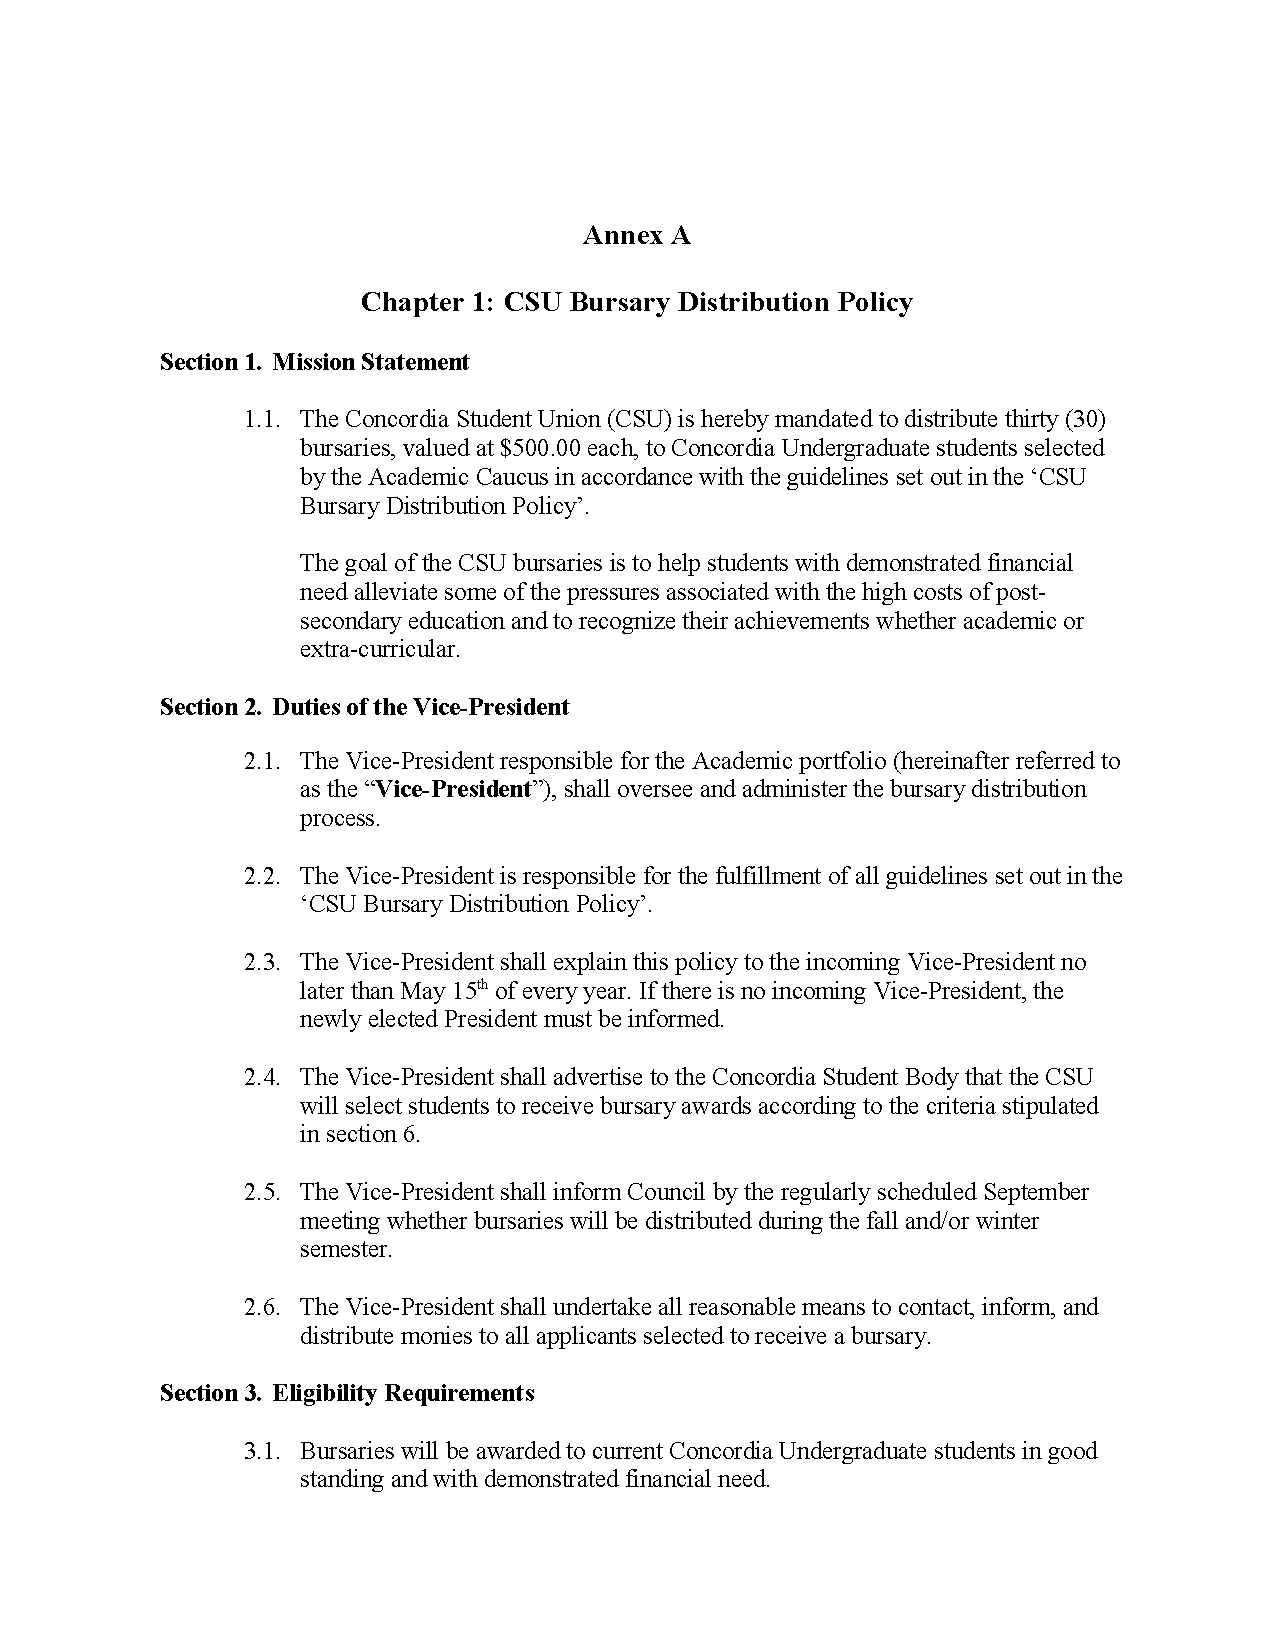
\includepdf[pages={-}]{annexes.pdf}
\end{document}
